% Version 2020-01-06
% update – 161114 by Ken Arroyo Ohori: made spacing closer to Word template throughout, put proper quotes everywhere, removed spacing that could cause labels to be wrong, added non-breaking and inter-sentence spacing where applicable, removed explicit newlines
% update – 010819 by Dennis Wittich: made spacing and font size closer to Word template, updated references and refernces style
% update – 042319 by Dennis Wittich: font size of captions set to 'small', first author names are shortened, hyphenation fixed
% update – 010620 by Dennis Wittich: Footnotes alignment set to left

\documentclass{isprs} % isprs class modified 23-04-2019 (Dennis Wittich)
\usepackage{subfigure}
\usepackage{setspace}
\usepackage{geometry} % added 27-02-2014 Markus Englich
\usepackage{epstopdf}
\usepackage{natbib}
\usepackage[colorlinks, allcolors=blue]{hyperref}
%\bibliographystyle{apalike}
\usepackage[labelsep=period]{caption}  % added 14-04-2016 Markus Englich - Recommendation by Sebastian Brocks
\usepackage[british]{babel} 
\usepackage[hang]{footmisc}
\def\footnotemargin{1em} % added 08-01-2020 Dennis Wittich
\usepackage{fancyref}

%\usepackage[authoryear]{natbib}
%\def\bibhang{0pt}

\geometry{a4paper, top=25mm, left=20mm, right=20mm, bottom=25mm, headsep=10mm, footskip=12mm} % added 27-02-2014 Markus Englich
%\usepackage{enumitem}

%\usepackage{isprs}
%\usepackage[perpage,para,symbol*]{footmisc}

%\renewcommand*{\thefootnote}{\fnsymbol{footnote}}
\captionsetup{justification=centering,font=normal} % thanks to Niclas Borlin 05-05-2016
\captionsetup[figure]{font=small} % added 23-04-2019 Dennis Wittich
\captionsetup[table]{font=small} % added 23-04-2019 Dennis Wittich

% Location of the images
\graphicspath{{figures/}}

\begin{document}

\title{Assessing Digital Elevation Models with different image overlap using photogrammetry}

% KAO: Remove extra spacing
\author{Robert van de Vlasakker}

% KAO: Remove extra newline
\address{} % Not needed

% If the corresponding author is NOT the final author, always add a % space before the subsequent comma, i.e.
% first author name\textsuperscript{a,}\thanks{Corresponding author} , % second author name \textsuperscript{b}, etc.
% thanks to Niclas Borlin 05-05-2016

% BB: leave these empty, but do not delete
\commission{}{} %This field is optional.
\workinggroup{} %This field is optional.
\icwg{}   %This field is optional.

% KAO: Use times symbol
\abstract{
Lorem ipsum dolor sit amet, consectetur adipiscing elit, sed do eiusmod tempor incididunt ut labore et dolore magna aliqua. Ut enim ad minim veniam, quis nostrud exercitation ullamco laboris nisi ut aliquip ex ea commodo consequat. Duis aute irure dolor in reprehenderit in voluptate velit esse cillum dolore eu fugiat nulla pariatur. Excepteur sint occaecat cupidatat non proident, sunt in culpa qui officia deserunt mollit anim id est laborum.
}

\keywords{Photogrammetry, Digital Elevation Model, Image Overlap}

\maketitle

%\saythanks % added 28-02-2014 Markus Englich

\section{Introduction}\label{Introduction}


Photogrammetry is the process of reconstructing spatial information with images through computer vision. 
The process uses similar points visible on multiple images to determine the points in space.
The reconstruction certainty of these points is strongly dependent on the overlap between different images. 
When a point is visible on more images, the reconstruction certainty we be higher.
This is especially the case with the reconstruction of irregular formed object like vegetation \citep{AccessingImageOverlap}.
With irregular objects, a higher overlap is preferred to capture each side of the object.
If parts of the object are not visible on the image, they will not be reconstructed in the point cloud.
So the overlap strongly influences the point cloud density in the dense cloud \citep{OptimalAltOverWeath}.
In the reconstruction process, a high overlap will also result in longer computation time \citep{AccessingImageOverlap}
However, a higher image overlap, does not automatically results in a higher point accuracy (x,y,z) \citep{EffectofUABimgcamover}.
By investigating how reducing the image overlap influences photogrammetry results, time and computing power may be saved without loosing too much spatial information.

With the development of cheap Unmanned Aerial Vehicles (UAV) photogrammetry has become more and more popular. 
UAV's come with high resolution cameras, GNSS and are available almost anywhere these days.
While UAV's do come with high resolution sensors and relatively cheap, small, high capacity batteries are not available \citep{UAVpopularity}.
A high image overlap takes longer to gather than a low image overlap. 
A drone can use a higher altitude so the sensor captures a larger area.
however, with a higher flight altitude the detail of the image will be less than that of a drone with a lower flight altitude.
This way the gathering process takes longer, and the UAV might even need to switch batteries instead of taking the images in a single flight.


\section{Materials and Methods}

\subsection{Study Area}\label{sec:Study Area}
The data covers an area in Ghana, about 20km south east of Ejura (lat. 7.3064212, lon. -1.164493). 
The area of interest is about 25000 m\textsuperscript{2}. 
The area consists mostly of sanvannah.
There are a few trees present.
\begin{figure}[htp]
    \centering
    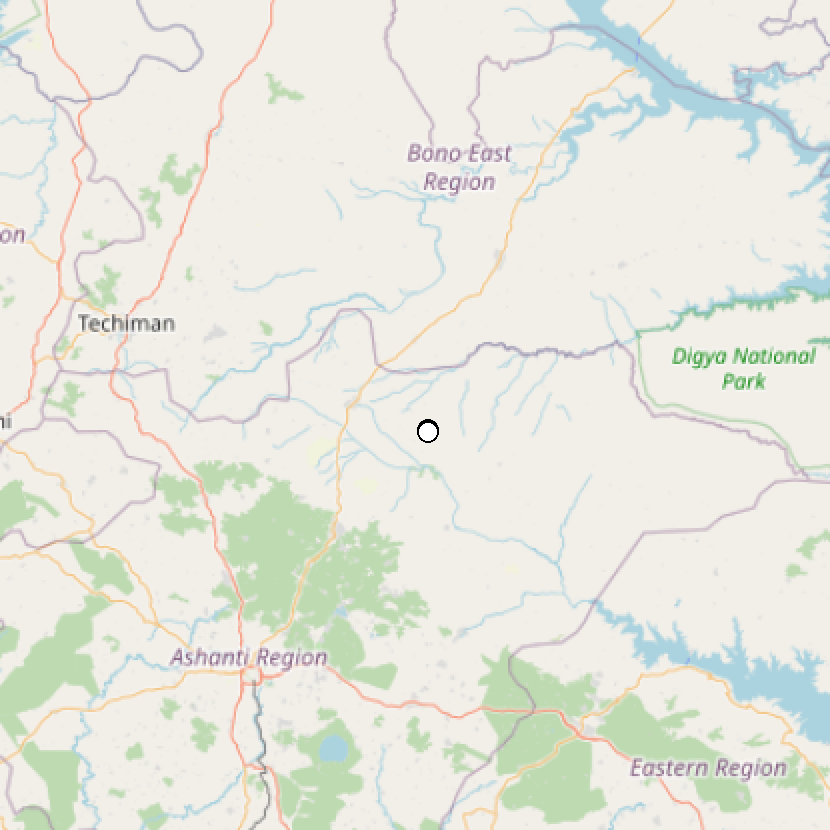
\includegraphics[width=4cm]{locationwide.png}
    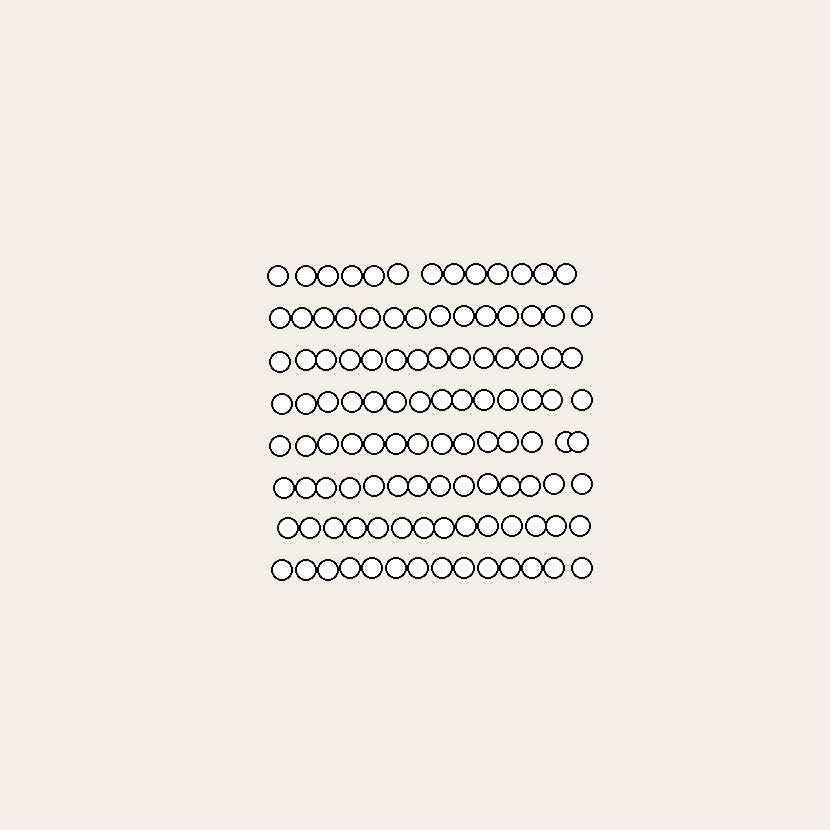
\includegraphics[width=4cm]{locationzoom.png}
    \caption{Area of Interest and Image Locations}
    \label{fig:areaofinterest}
\end{figure}
Each image has a resolution of 4000 times 3000 and was taken by a DJI Phantom 3.
The images all contain GNNS location (WGS84). 
Their exact location can be found in figure \ref{fig:areaofinterest}.


\subsection{Image Selection and Processing}
For image processing and DEM generation Agisoft Metashape Professional edition 1.6.5 (Agisoft LLC., St. Peterburg, Russia) was used.
First, the complete data set has been aligned on medium quality.
Next, the dense cloud was built on medium quality (no depth filtering), resulting in a dense cloud of 3,268,264 points.



The generation of three-dimensional (3D) dense point clouds from the images were performed for each acquisition using the proprietary software Agisoft Photoscan Professional version 1.1 (Agisoft LLC., St. Petersburg, Russia)

\subsection{DEM}

% KAO: Sloppy spacing ensures non-overfull lines. Can be removed if this is not an issue.
\sloppy




{
	\begin{spacing}{1.17}
		\normalsize
		\bibliography{bibliography} % Include your own bibliography (*.bib), style is given in isprs.cls
	\end{spacing}
}



\vspace{1cm}
\end{document}
